% Chapitre 19 -- G-AUTOEVOLVE : AutoevolveAI / ANSE, le banc d'essai construit pour que les fausses affirmations échouent
% Sources : results/discovery_journal_2026/TOP20.json (pick 19) ; github_inventory.md (AutoevolveAI) ; README.md du dépôt
% (« The problem this project is actually about », « Measured status », exemple Störmer-Verlet) ;
% docs/remediation/AUDIT_2026-09-25.md (section 2) et AUDIT_2026-09-26.md (section 0).
% Démonstration en direct : code/fig19.py
% (anse/formal/lean_runner.py sur cinq fichiers). Figure : code/fig19.py.
\chapter[Le banc qui s'inspecte]{Le banc d'essai qui s'est inspecté lui-même}
\reference{Dépôt public AutoevolveAI, créé le 19 septembre 2026. Audits internes des 25 et 26 septembre 2026. Pas de DOI propre.}

\noindent\niveau{C} pour ce que l'on dit du banc~: ce sont des audits internes et des raisonnements, pas des
preuves vérifiées par une machine.

\section*{L'idée en une image}

\begin{analogie}
Une cuisine fait sa propre inspection et découvre des fours qui affichent \og cuit\fg{} sans avoir chauffé, et un
thermomètre qui indique toujours la bonne température. Avant de cuisiner à nouveau, elle répare les thermomètres,
et elle prend une règle~: un thermomètre ne compte que si on l'a vu, au moins une fois, signaler un four froid.

\emph{Où l'image cesse d'être juste~:} ici les inspecteurs étaient des agents d'IA du même projet, pas un service
d'hygiène indépendant~; et même un bon thermomètre ne dit pas si le plat est bon~: un énoncé vide de sens passe
encore les contrôles, comme on le verra.
\end{analogie}

\section*{Ce qui a été fait}

AutoevolveAI est l'établi du projet~: le logiciel qui fait tourner les modèles de langage installés sur la machine,
les vérifications Lean, les calculs sur la carte graphique, le registre des affirmations et les scripts de
publication utilisés par les articles de l'automne. Fin septembre, des audits internes, menés par des agents d'IA
sous la direction de l'auteur, ont trouvé \textbf{14 composants qui annonçaient un succès sans avoir fait le
travail}. Quelques exemples, publiés dans le dépôt~:
\begin{itemize}
\item un module de mesure de la carte graphique renvoyait des nombres tirés au hasard, présentés comme la
  \og vérité physique\fg~;
\item un entraînement nocturne qui n'avait rien entraîné était enregistré comme un modèle déployé~;
\item un script de \og relecture par les pairs\fg{} écrivait \og accepté sans réserve\fg{} sans jamais appeler de
  relecteur~;
\item un juge des preuves Lean cherchait le mot \og error\fg{} au mauvais endroit, là où Lean n'écrit pas ses
  erreurs, et acceptait donc presque tout~;
\item un modèle affiné était étiqueté \og succès\fg{} alors que son erreur avait augmenté, de $3{,}532$ à $3{,}692$.
\end{itemize}
Le lendemain, l'audit a trouvé pire, et l'a écrit~: une version publiée du banc annonçait que les correctifs
étaient en place et que les contrôles passaient. Aucun des deux n'était vrai~; le contrôle échouait, mais son code
d'échec avait été masqué par un tuyau de commandes qui ne transmettait que le code du dernier programme.

De là vient la règle du projet~: \emph{toute affirmation chiffrée doit remonter à un fichier, et tout contrôle doit
pouvoir échouer. Un contrôle qui n'a jamais rien refusé n'est pas un contrôle.}

\paragraph{Un exemple à suivre au crayon.} Le seul juge Lean sûr du banc compile le fichier, puis demande au noyau
la liste des axiomes de chaque théorème. Nous l'avons fait tourner, pour ce livre, sur cinq petits fichiers
(figure~\ref{fig:c19}). Une preuve honnête de $n+0=n$~; la même \og prouvée\fg{} par le trou \texttt{sorry}~; $1=2$
tiré d'un axiome inventé~; un théorème qui affirme seulement \og Vrai\fg~; et $1=2$ \og prouvé\fg{} par simple calcul.
Les quatre premiers se compilent avec le code de sortie~$0$~: un juge naïf les accepte tous. Le juge du banc lit
\texttt{sorryAx} dans le deuxième et \texttt{cheat} dans le troisième, et les refuse. Le cinquième ne compile pas.
Mais le quatrième, qui ne dit rien, est accepté~: c'est la limite du thermomètre.

\section*{Comment on s'est assuré que ce n'est pas faux}

Les constats sont décrits fichier par fichier et ligne par ligne dans les deux rapports d'audit publics, et chacun
peut les relire dans le code. L'audit lui-même a été corrigé quand les faits l'ont contredit~: deux de ses
affirmations (des fichiers dits inventés, des poids dits absents) se sont révélées fausses, et la correction est
consignée. Une leçon plus fine est venue d'une relecture automatique~: un relecteur qui refuse tout réussit le test
\og il doit refuser un mauvais article\fg{} sans rien savoir~; le banc a donc ajouté le contrôle inverse, un article
trivialement correct qui doit être accepté. Un contrôle négatif seul n'est qu'une moitié de validation. Rien de tout
cela n'a été relu par un humain extérieur.

\section*{Ce que ça ne dit pas}

\begin{limite}
\begin{itemize}
\item Ce sont des audits internes~: le projet s'est inspecté lui-même, avec des agents d'IA.
\item Le banc n'est pas \og réparé\fg~: selon son propre README, mesuré à la version~13.2.1, 1\,371 tests passent,
  15 échouent et 8 sont en erreur, et une liste publique des défauts connus sert de feuille de route.
\item L'audit des axiomes ne voit pas un énoncé vide ou mal choisi~; seule la relecture de l'énoncé le peut, et
  c'est l'étape que l'année n'a pas encore faite avec un humain.
\item Un banc qui refuse les fausses preuves ne produit pas de vraies découvertes~; il empêche seulement certaines
  erreurs d'en avoir l'air.
\end{itemize}
\end{limite}

\section*{Pour aller plus loin}

Le dépôt public AutoevolveAI contient le code, le README avec sa section d'état mesuré et ses défauts connus, et
les rapports d'audit des 25 et 26 septembre 2026 dans \texttt{docs/remediation}.

\begin{figure}[t]
\centering
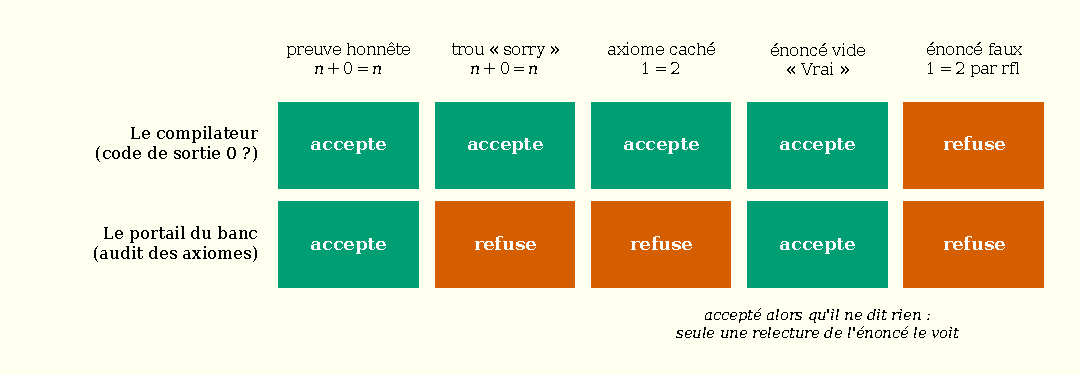
\includegraphics[width=\linewidth]{figures/c19_portail}
\caption{Cinq fichiers Lean passés pour ce livre au juge du banc. En haut, ce que dit le seul code de sortie~; en bas,
le verdict après audit des axiomes. L'énoncé vide est accepté par les deux.}
\label{fig:c19}
\end{figure}
